


\tikzset{every picture/.style={line width=0.75pt}} %set default line width to 0.75pt        

\begin{tikzpicture}[x=0.75pt,y=0.75pt,yscale=-1,xscale=1]
%uncomment if require: \path (0,300); %set diagram left start at 0, and has height of 300

%Image [id:dp9645385719858803] 
\draw (328.5,141.07) node  {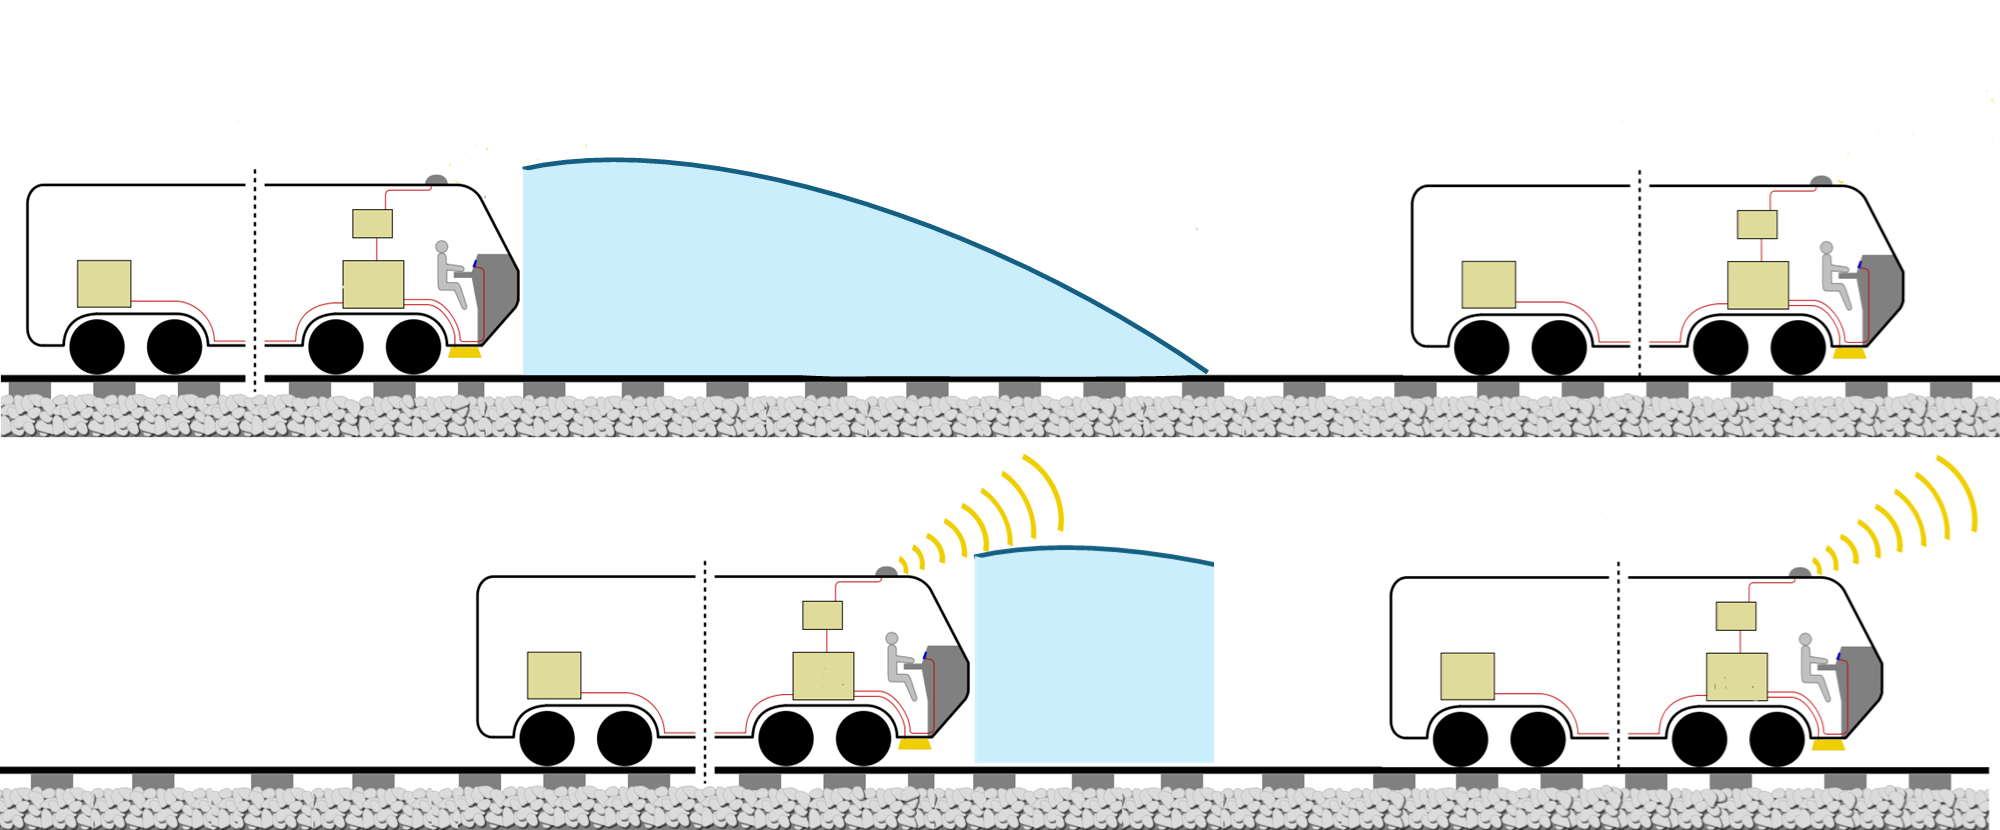
\includegraphics[width=623.25pt,height=272.36pt]{Part3/figure/levels.png}};
%Straight Lines [id:da2569807320997002] 
\draw [line width=3]    (426.2,116.9) -- (493.2,116.9) ;
\draw [shift={(493.2,116.9)}, rotate = 180] [color={rgb, 255:red, 0; green, 0; blue, 0 }  ][line width=3]    (0,8.94) -- (0,-8.94)   ;
\draw [shift={(426.2,116.9)}, rotate = 180] [color={rgb, 255:red, 0; green, 0; blue, 0 }  ][line width=3]    (0,8.94) -- (0,-8.94)   ;
%Rounded Rect [id:dp5947681861561565] 
\draw  [fill={rgb, 255:red, 248; green, 231; blue, 28 }  ,fill opacity=1 ] (-32,3.3) .. controls (-32,-0.18) and (-29.18,-3) .. (-25.7,-3) -- (9.7,-3) .. controls (13.18,-3) and (16,-0.18) .. (16,3.3) -- (16,22.2) .. controls (16,25.68) and (13.18,28.5) .. (9.7,28.5) -- (-25.7,28.5) .. controls (-29.18,28.5) and (-32,25.68) .. (-32,22.2) -- cycle ;
%Rounded Rect [id:dp6734872499020808] 
\draw  [fill={rgb, 255:red, 248; green, 231; blue, 28 }  ,fill opacity=1 ] (-26,192.97) .. controls (-26,189.49) and (-23.18,186.67) .. (-19.7,186.67) -- (15.7,186.67) .. controls (19.18,186.67) and (22,189.49) .. (22,192.97) -- (22,211.87) .. controls (22,215.35) and (19.18,218.17) .. (15.7,218.17) -- (-19.7,218.17) .. controls (-23.18,218.17) and (-26,215.35) .. (-26,211.87) -- cycle ;
%Straight Lines [id:da009919353756201676] 
\draw [line width=3]    (421.53,277.57) -- (488.53,277.57) ;
\draw [shift={(488.53,277.57)}, rotate = 180] [color={rgb, 255:red, 0; green, 0; blue, 0 }  ][line width=3]    (0,8.94) -- (0,-8.94)   ;
\draw [shift={(421.53,277.57)}, rotate = 180] [color={rgb, 255:red, 0; green, 0; blue, 0 }  ][line width=3]    (0,8.94) -- (0,-8.94)   ;

% Text Node
\draw (-6.27,5.95) node   [align=left] {\begin{minipage}[lt]{25.98pt}\setlength\topsep{0pt}
{\LARGE {\fontfamily{ptm}\selectfont L3}}
\end{minipage}};
% Text Node
\draw (-4.67,196.95) node   [align=left] {\begin{minipage}[lt]{25.98pt}\setlength\topsep{0pt}
{\LARGE {\fontfamily{ptm}\selectfont VC}}
\end{minipage}};



\end{tikzpicture}
